% jak to bude vypadat
Pro potřeby zobrazení jsem se rozhodl vytvořit velmi jednoduchou \gls{spa}. Jediné co se na ní bude nacházet budou tři 
tlačítka pro přepínání mezi jednotlivými senzory a místo pro graf hodnot. Celá aplikace bude napsaná v javascriptu. 
Nejsem v něm úplně zběhlý, takže je možné, že některé konstrukce budou neoptimální nebo přinejmenším podivné, avšak 
nemělo by to mít vliv na funkčnost. Koncept celé aplikace vypadá takto.

\begin{figure}[H]
  \centering
  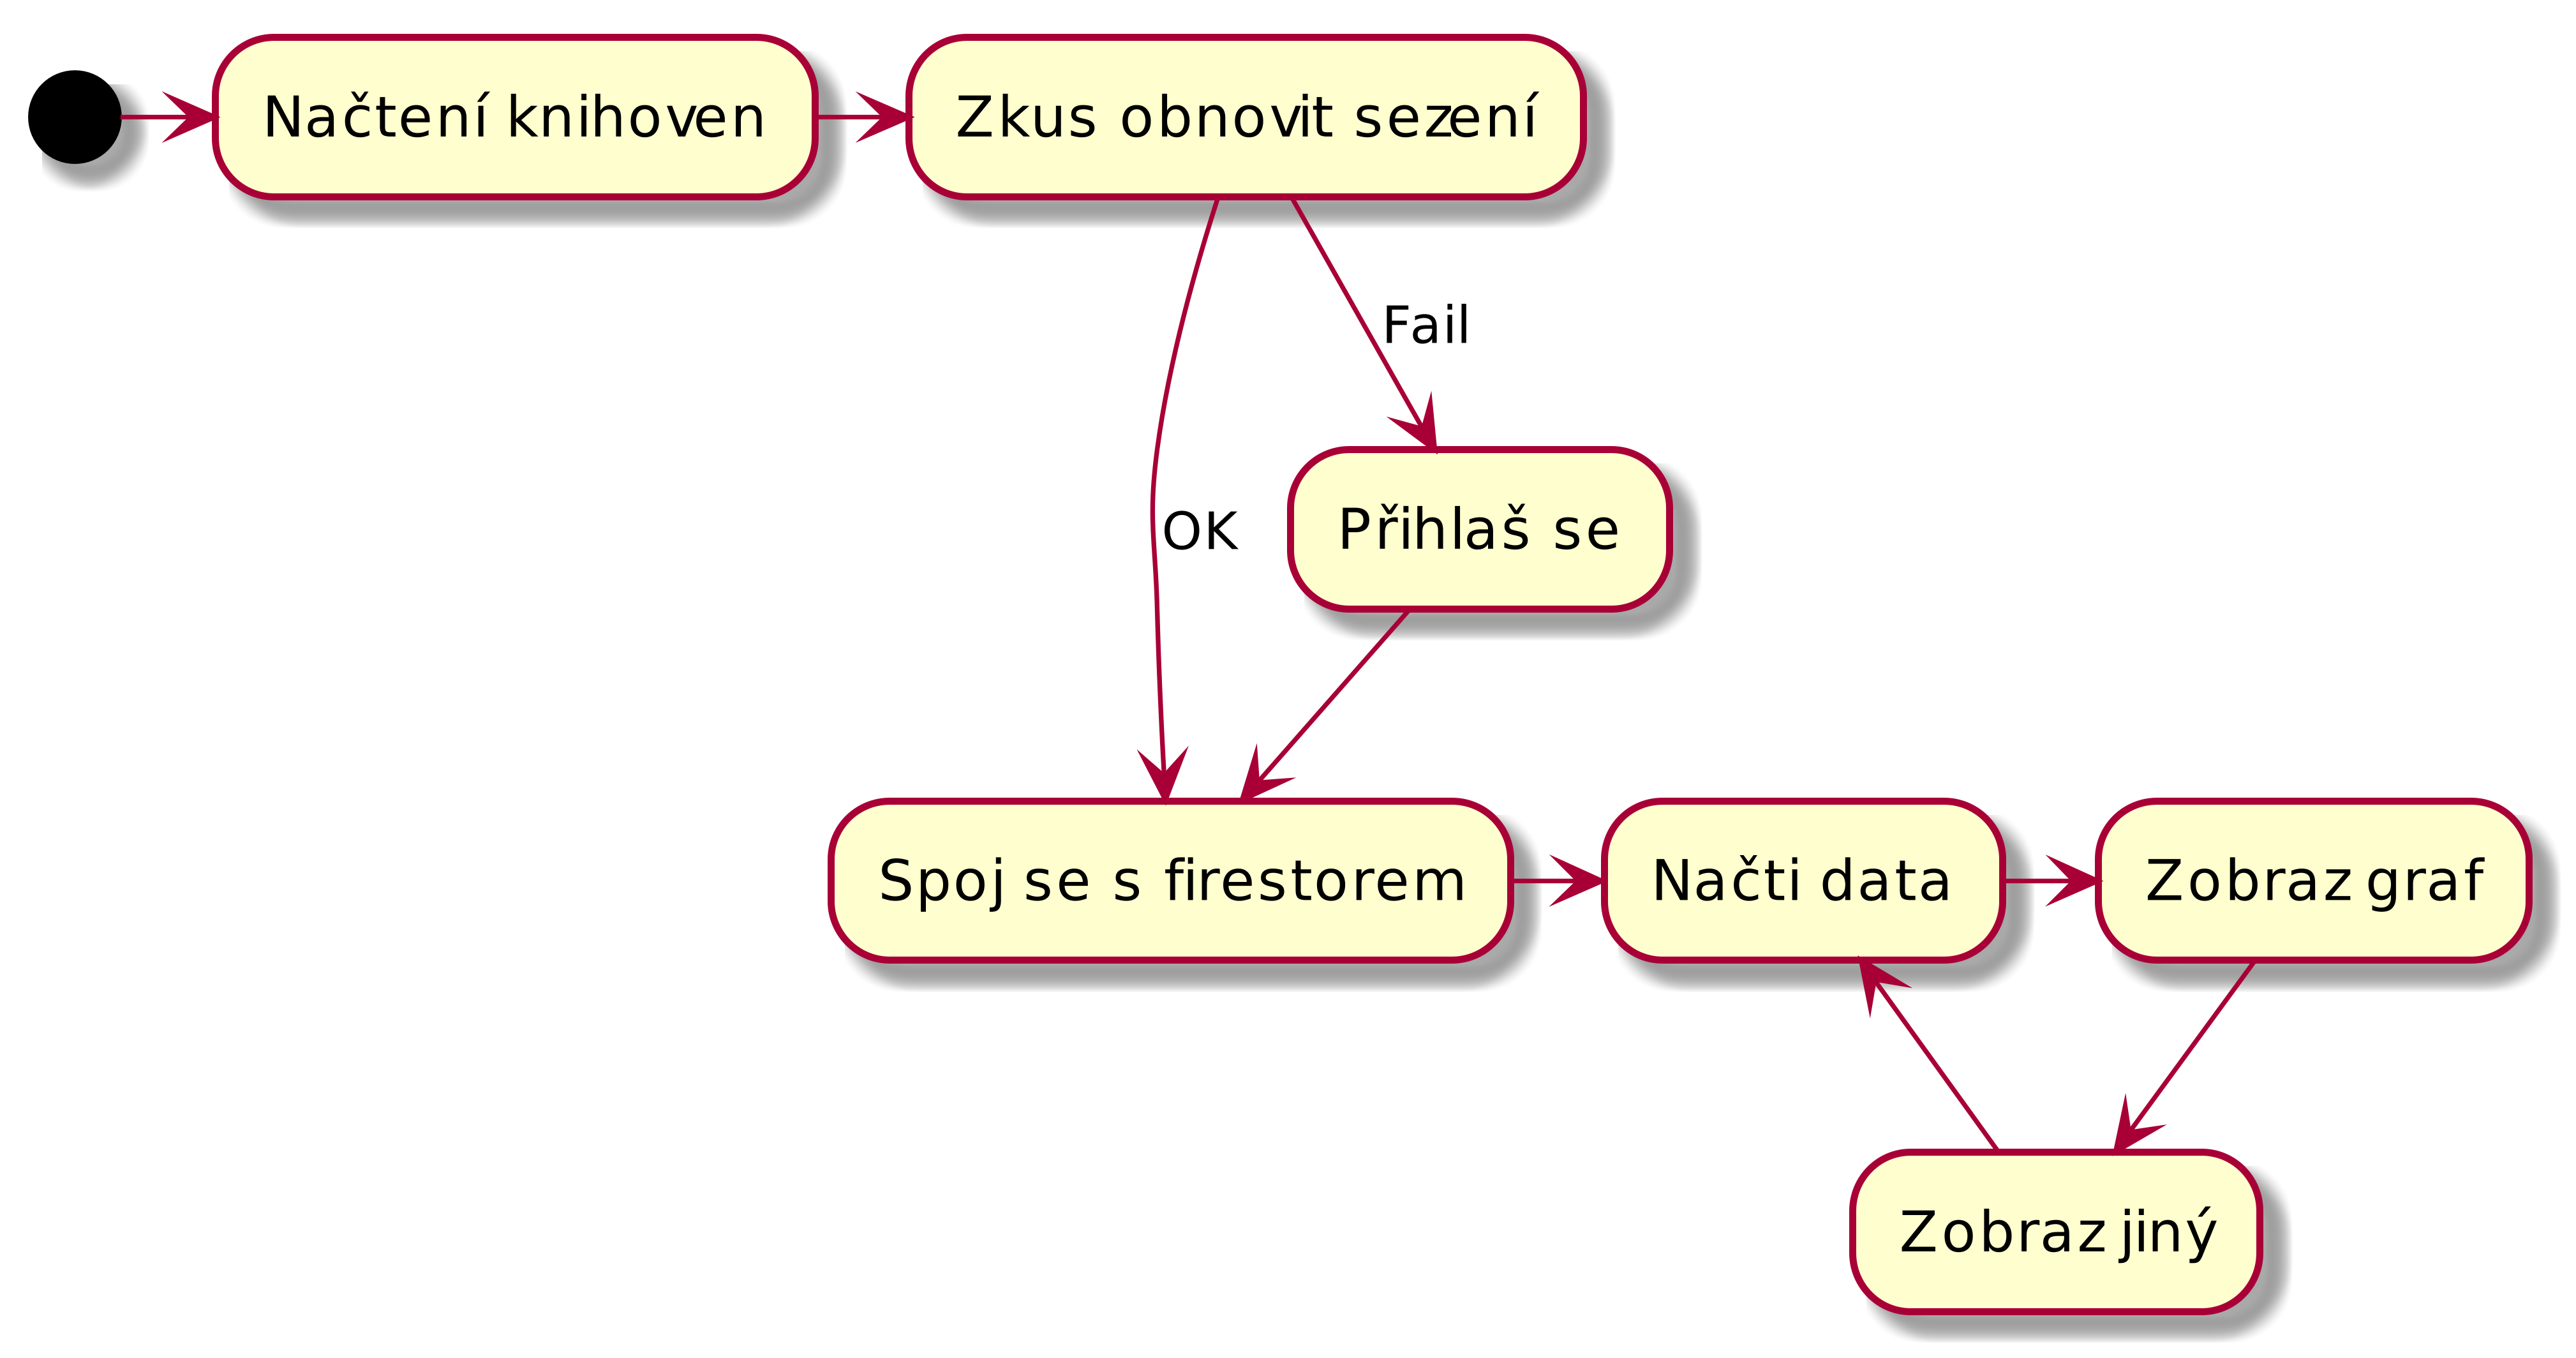
\includegraphics[width=\textwidth]{grafy.png}
  \caption{Průběh programu}
\end{figure}

Na začátku webové stránky, která tvoří kostru celého programu, načtu \gls{firebase} \glslink{knihovna}{knihovny}. 
Vzhledem k tomu, že používám \gls{firebase} hosting, je tato část velmi jednoduchá, neb nemusím řešit autorizace\ldots 
Poté načtu \glslink{knihovna}{knihovnu} \gls{plotly}, kterou používám pro vykreslování grafů. Následně vytvořím 
přepínací tlačítka a plochu pro graf. Nakonec zavolám funkci, co mi vykreslí graf hodnot v teráriu.

Do \gls{firebase} se přihlásím za použití \gls{oauth} u Googlu a to z jediného důvodu. Při nastavování Firestoru jsem 
nastavil pravidla tak, že bez přihlášení nikoho k datům nepustí. Takže jsem potřeboval nějak ověřit uživatele. Druhý 
problém byl, jak přesvědčit databázi, aby mi umožnila přístup k datům. Tady jsem použil místo řešení problémů 
s účty\ldots takový špinavý trik. Po přihlášení mi Google přidělil identifikátor, kterým se prokazuji vůči aplikaci, 
když jsem do pravidel přidal podmínku, že tento identifikátor může číst data, vše fungovalo. Není to řešení pro více 
uživatelů, ale dostačuje.

Následné vykreslení grafů už je v podstatě jen otázka, jak převést data z \gls{firebase} do pole. Začnu tím, že vyberu 
správnou kolekci dle použitého senzoru, tu si seřadím podle \glslink{timestamp}{timestampu} a z ní vezmu posledních 192 
hodnot, což odpovídá cca posledním 48 hodinám. Následně pouze proiteruji přes všechna data a přidám je do pole hodnot, 
jediná výjimka je u času, který před tím převedu na čitelný tvar a do aktuálního časového pásma. Pak už data v poli 
pouze předám \glslink{knihovna}{knihovně} \gls{plotly}, která je vykreslí. Když mám v jednom grafu více datových polí, 
vykresluji je nad sebe se stejnou časovou osou, abych mohl porovnávat odpovídající hodnoty. Výsledek pak vypadá nějak 
takto.

% obrázky grafů
% BME280
\begin{figure}[H]
    \centering
    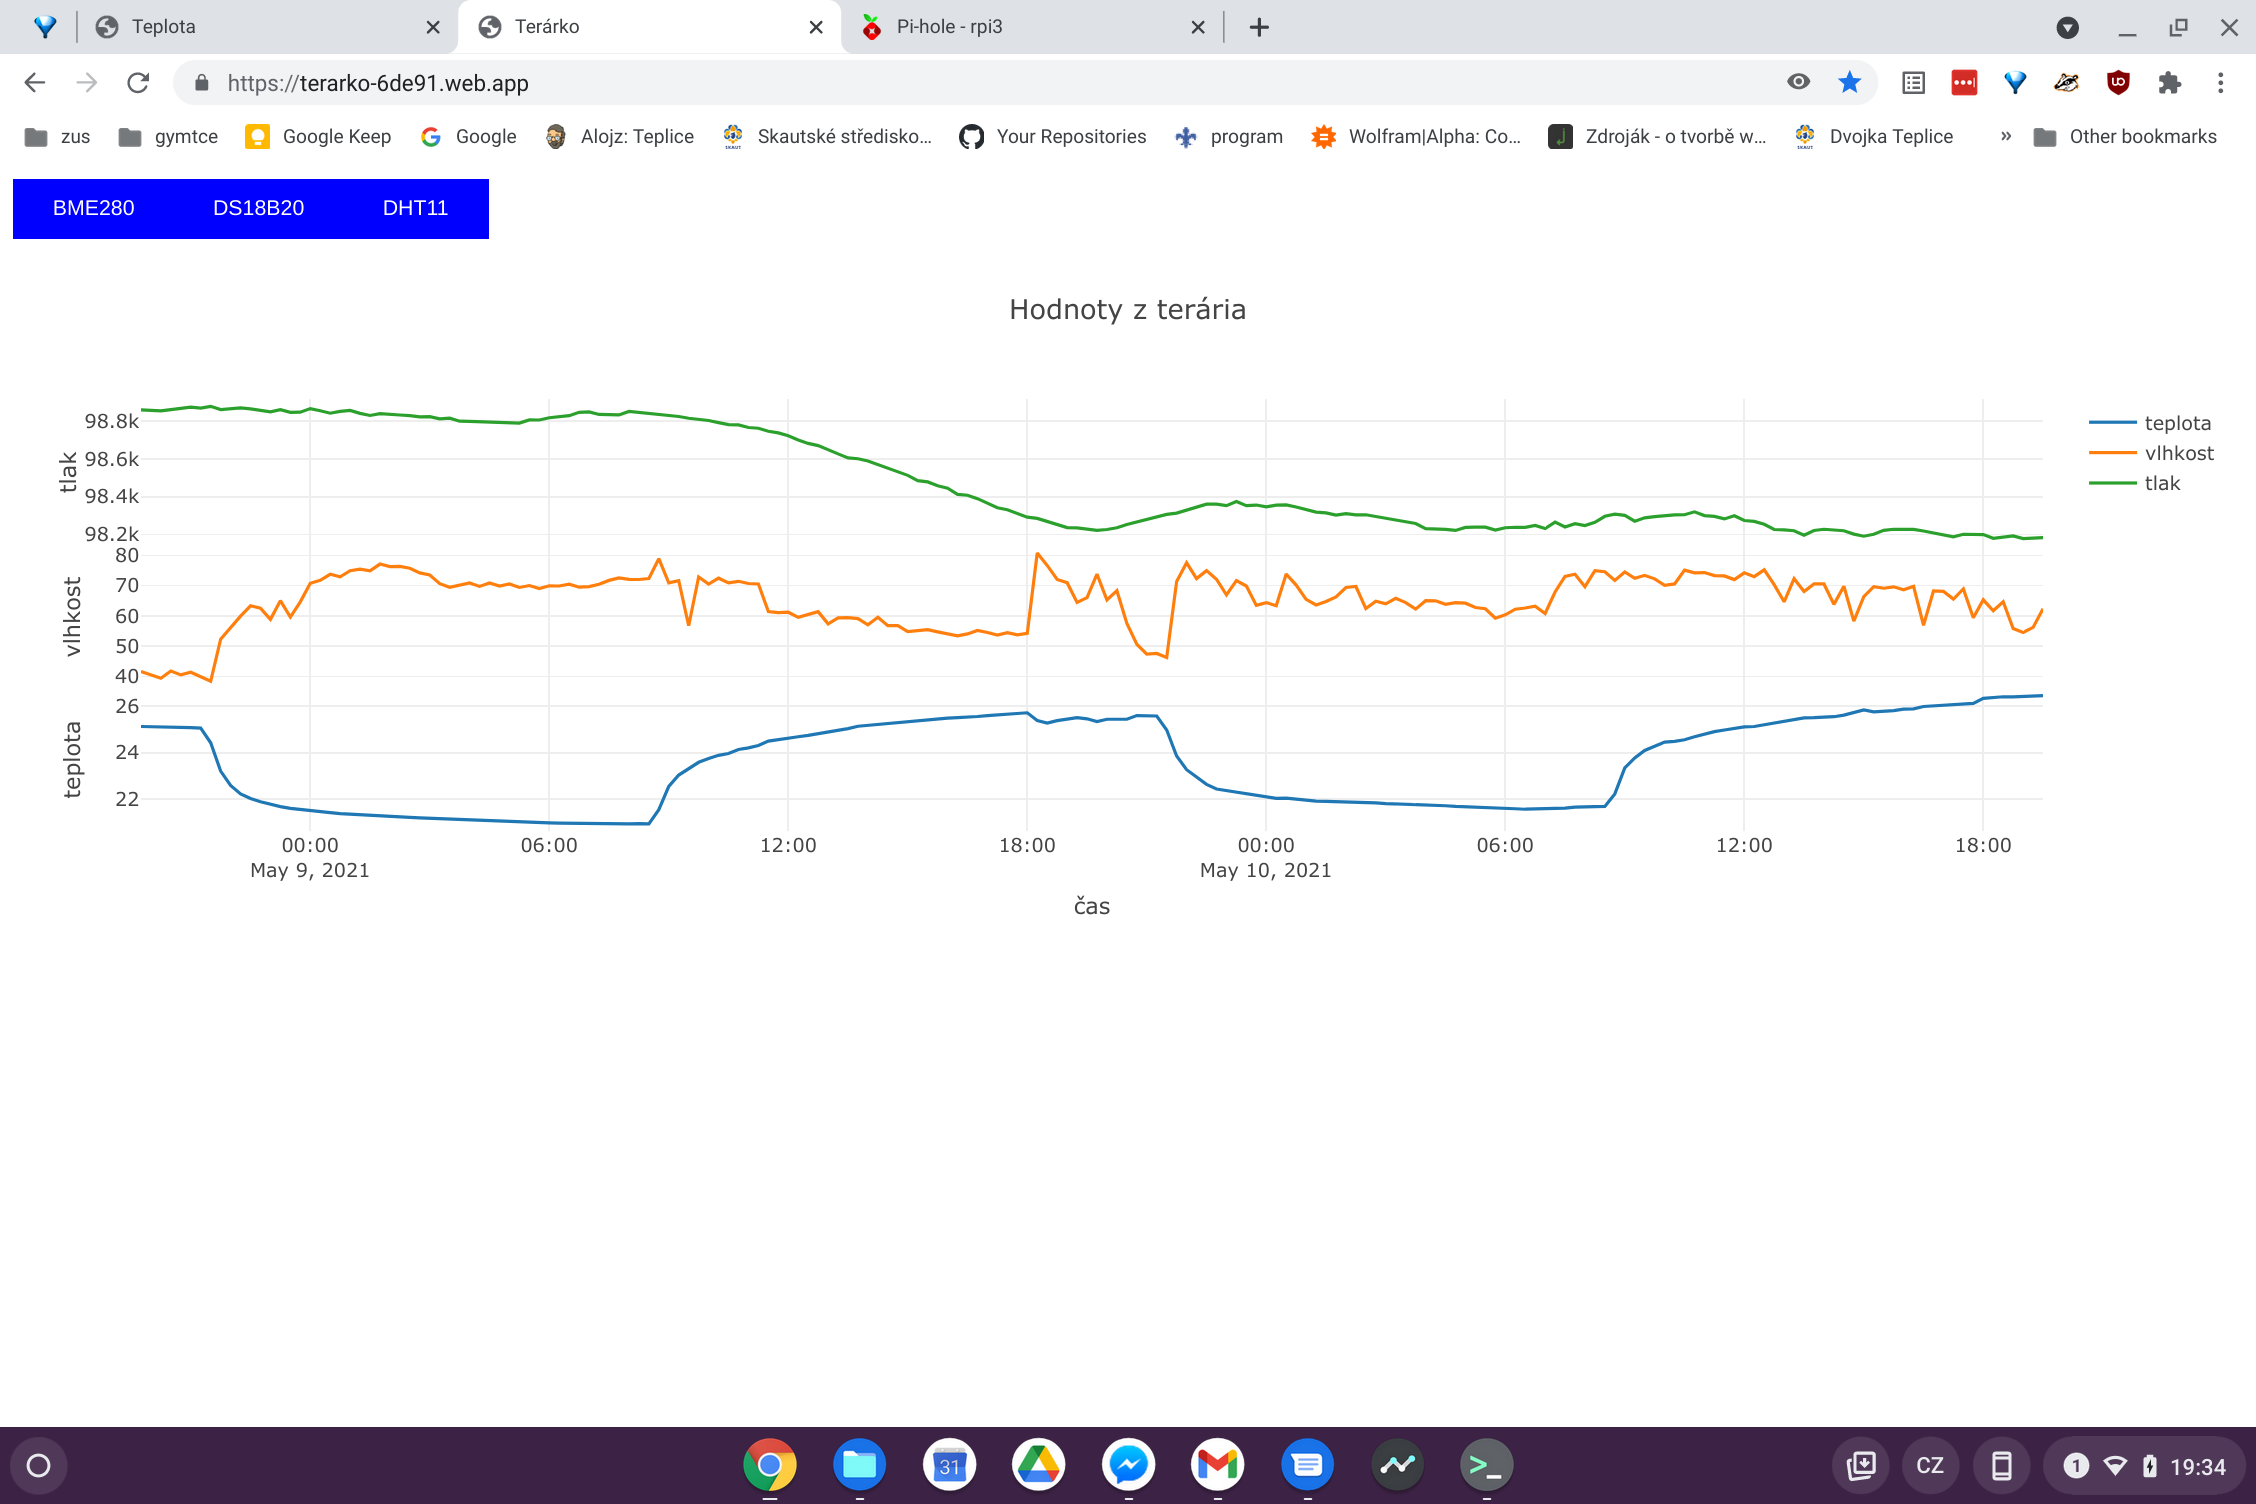
\includegraphics[width=0.8\textwidth]{BME280-graf.png}
    \caption{Data z terária}
\end{figure}
% DS18B20
\begin{figure}[H]
    \centering
    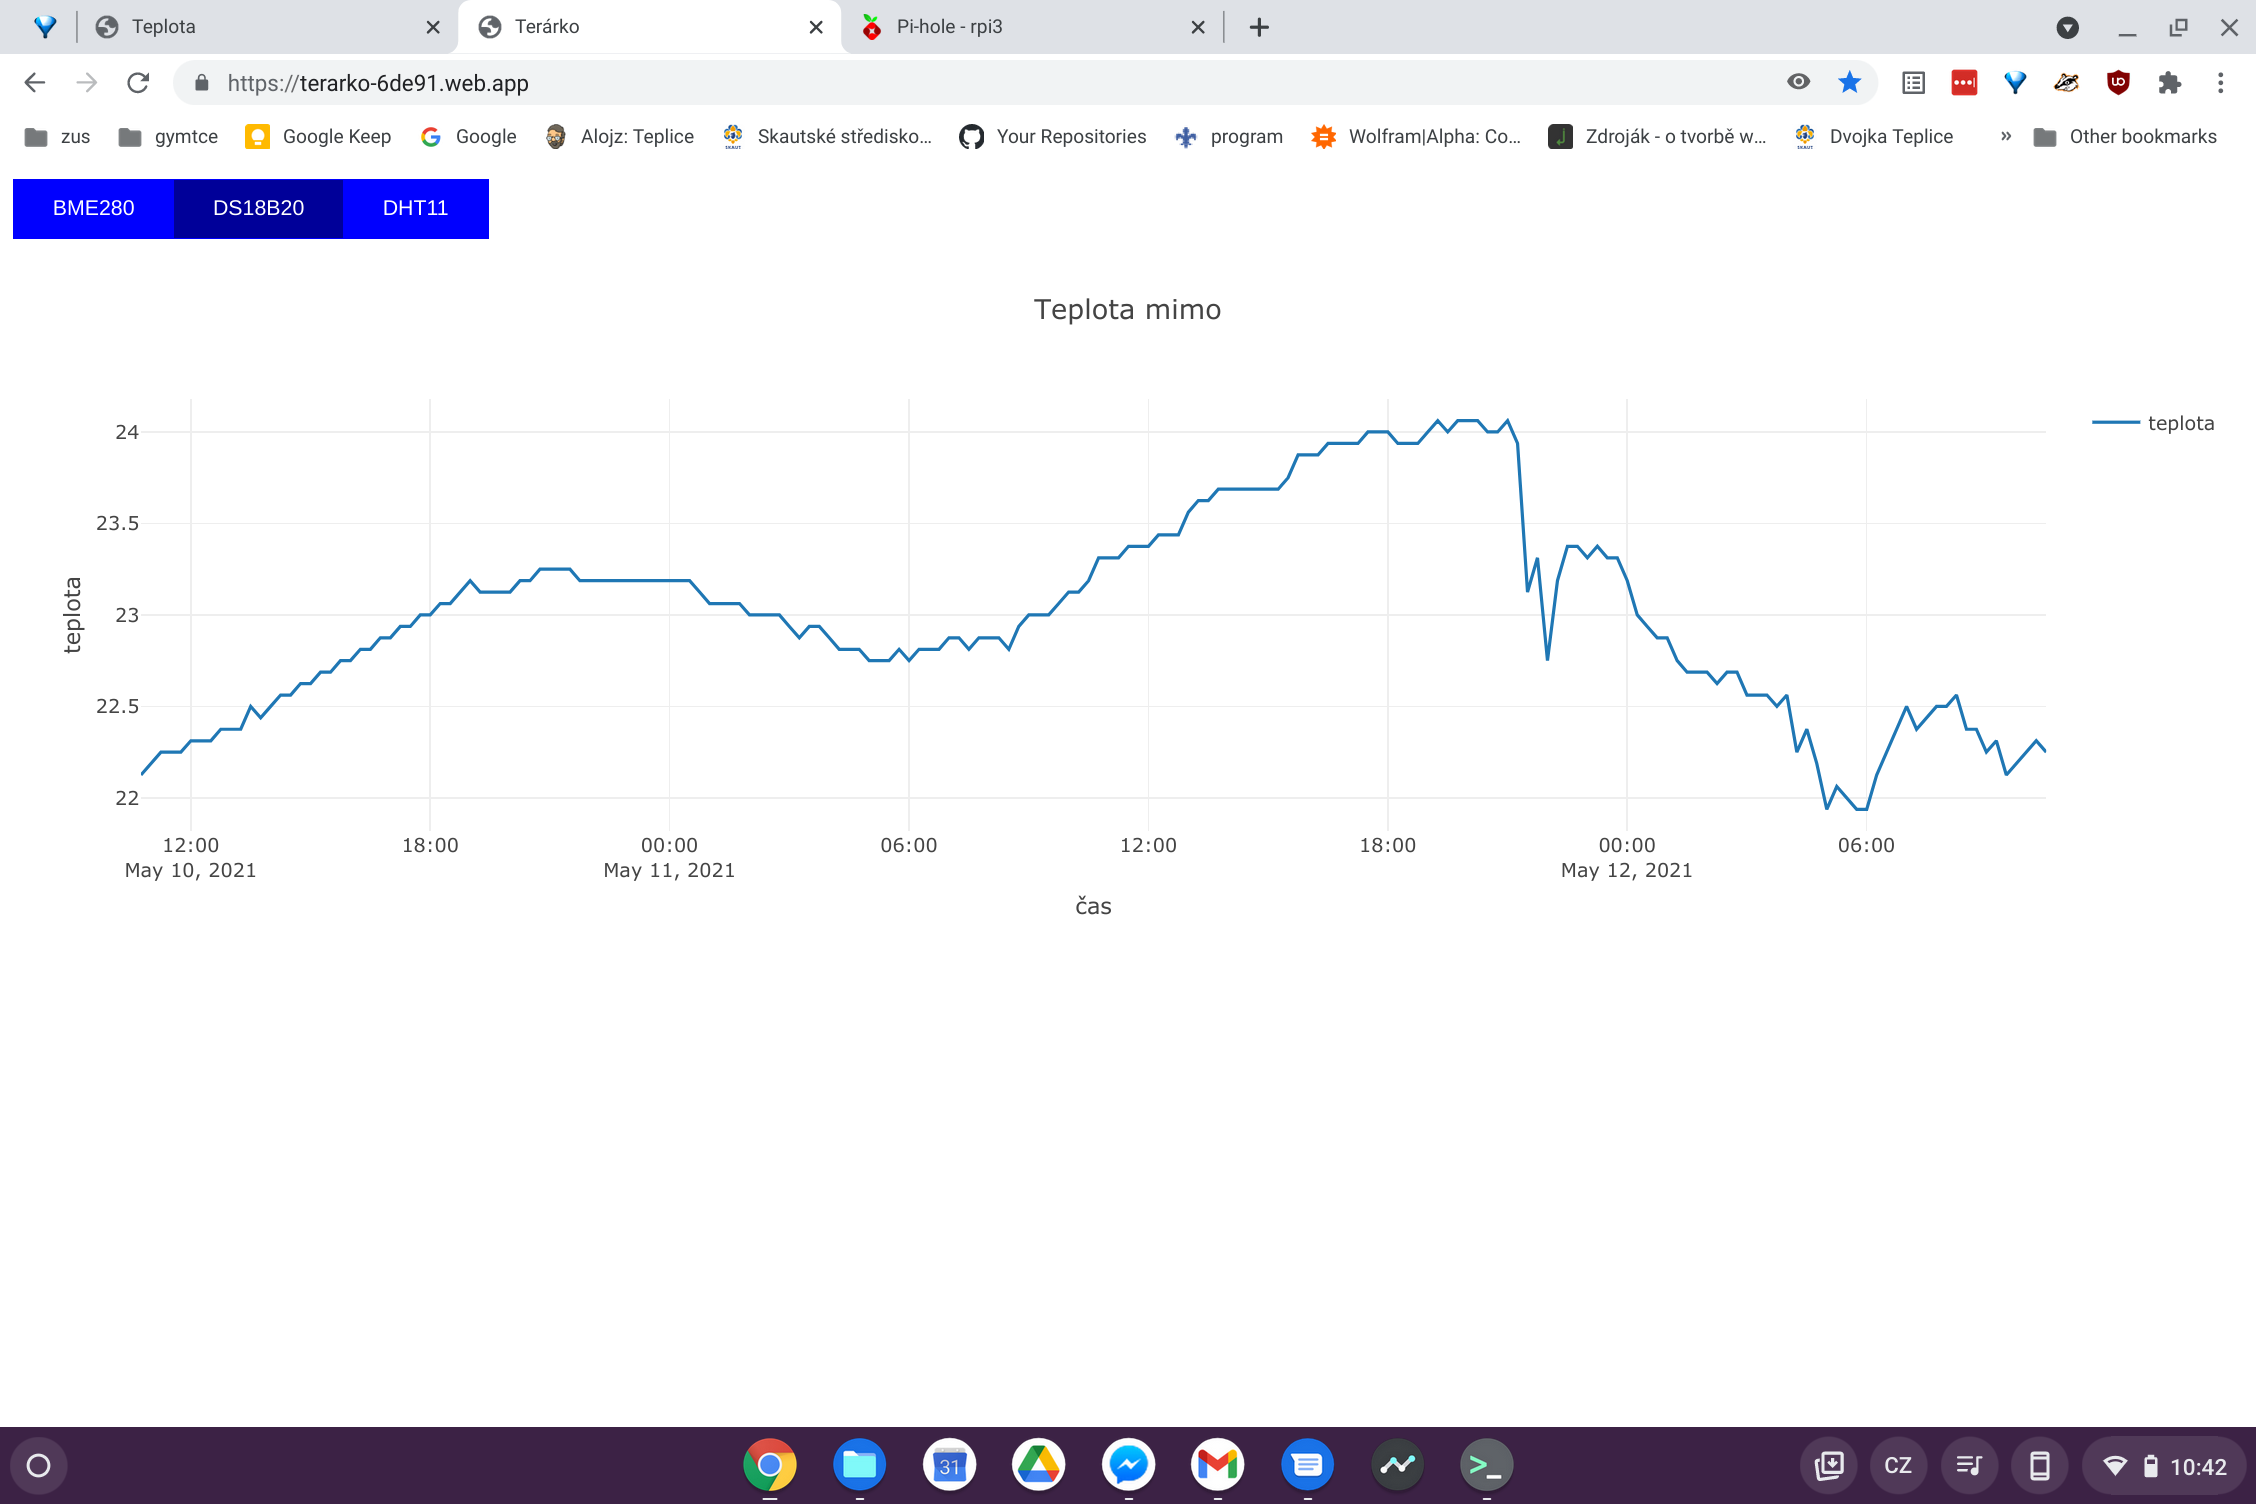
\includegraphics[width=0.8\textwidth]{DS18B20-graf.png}
    \caption{Teplota mimo terárium}
\end{figure}
% DHT11
\begin{figure}[H]
    \centering
    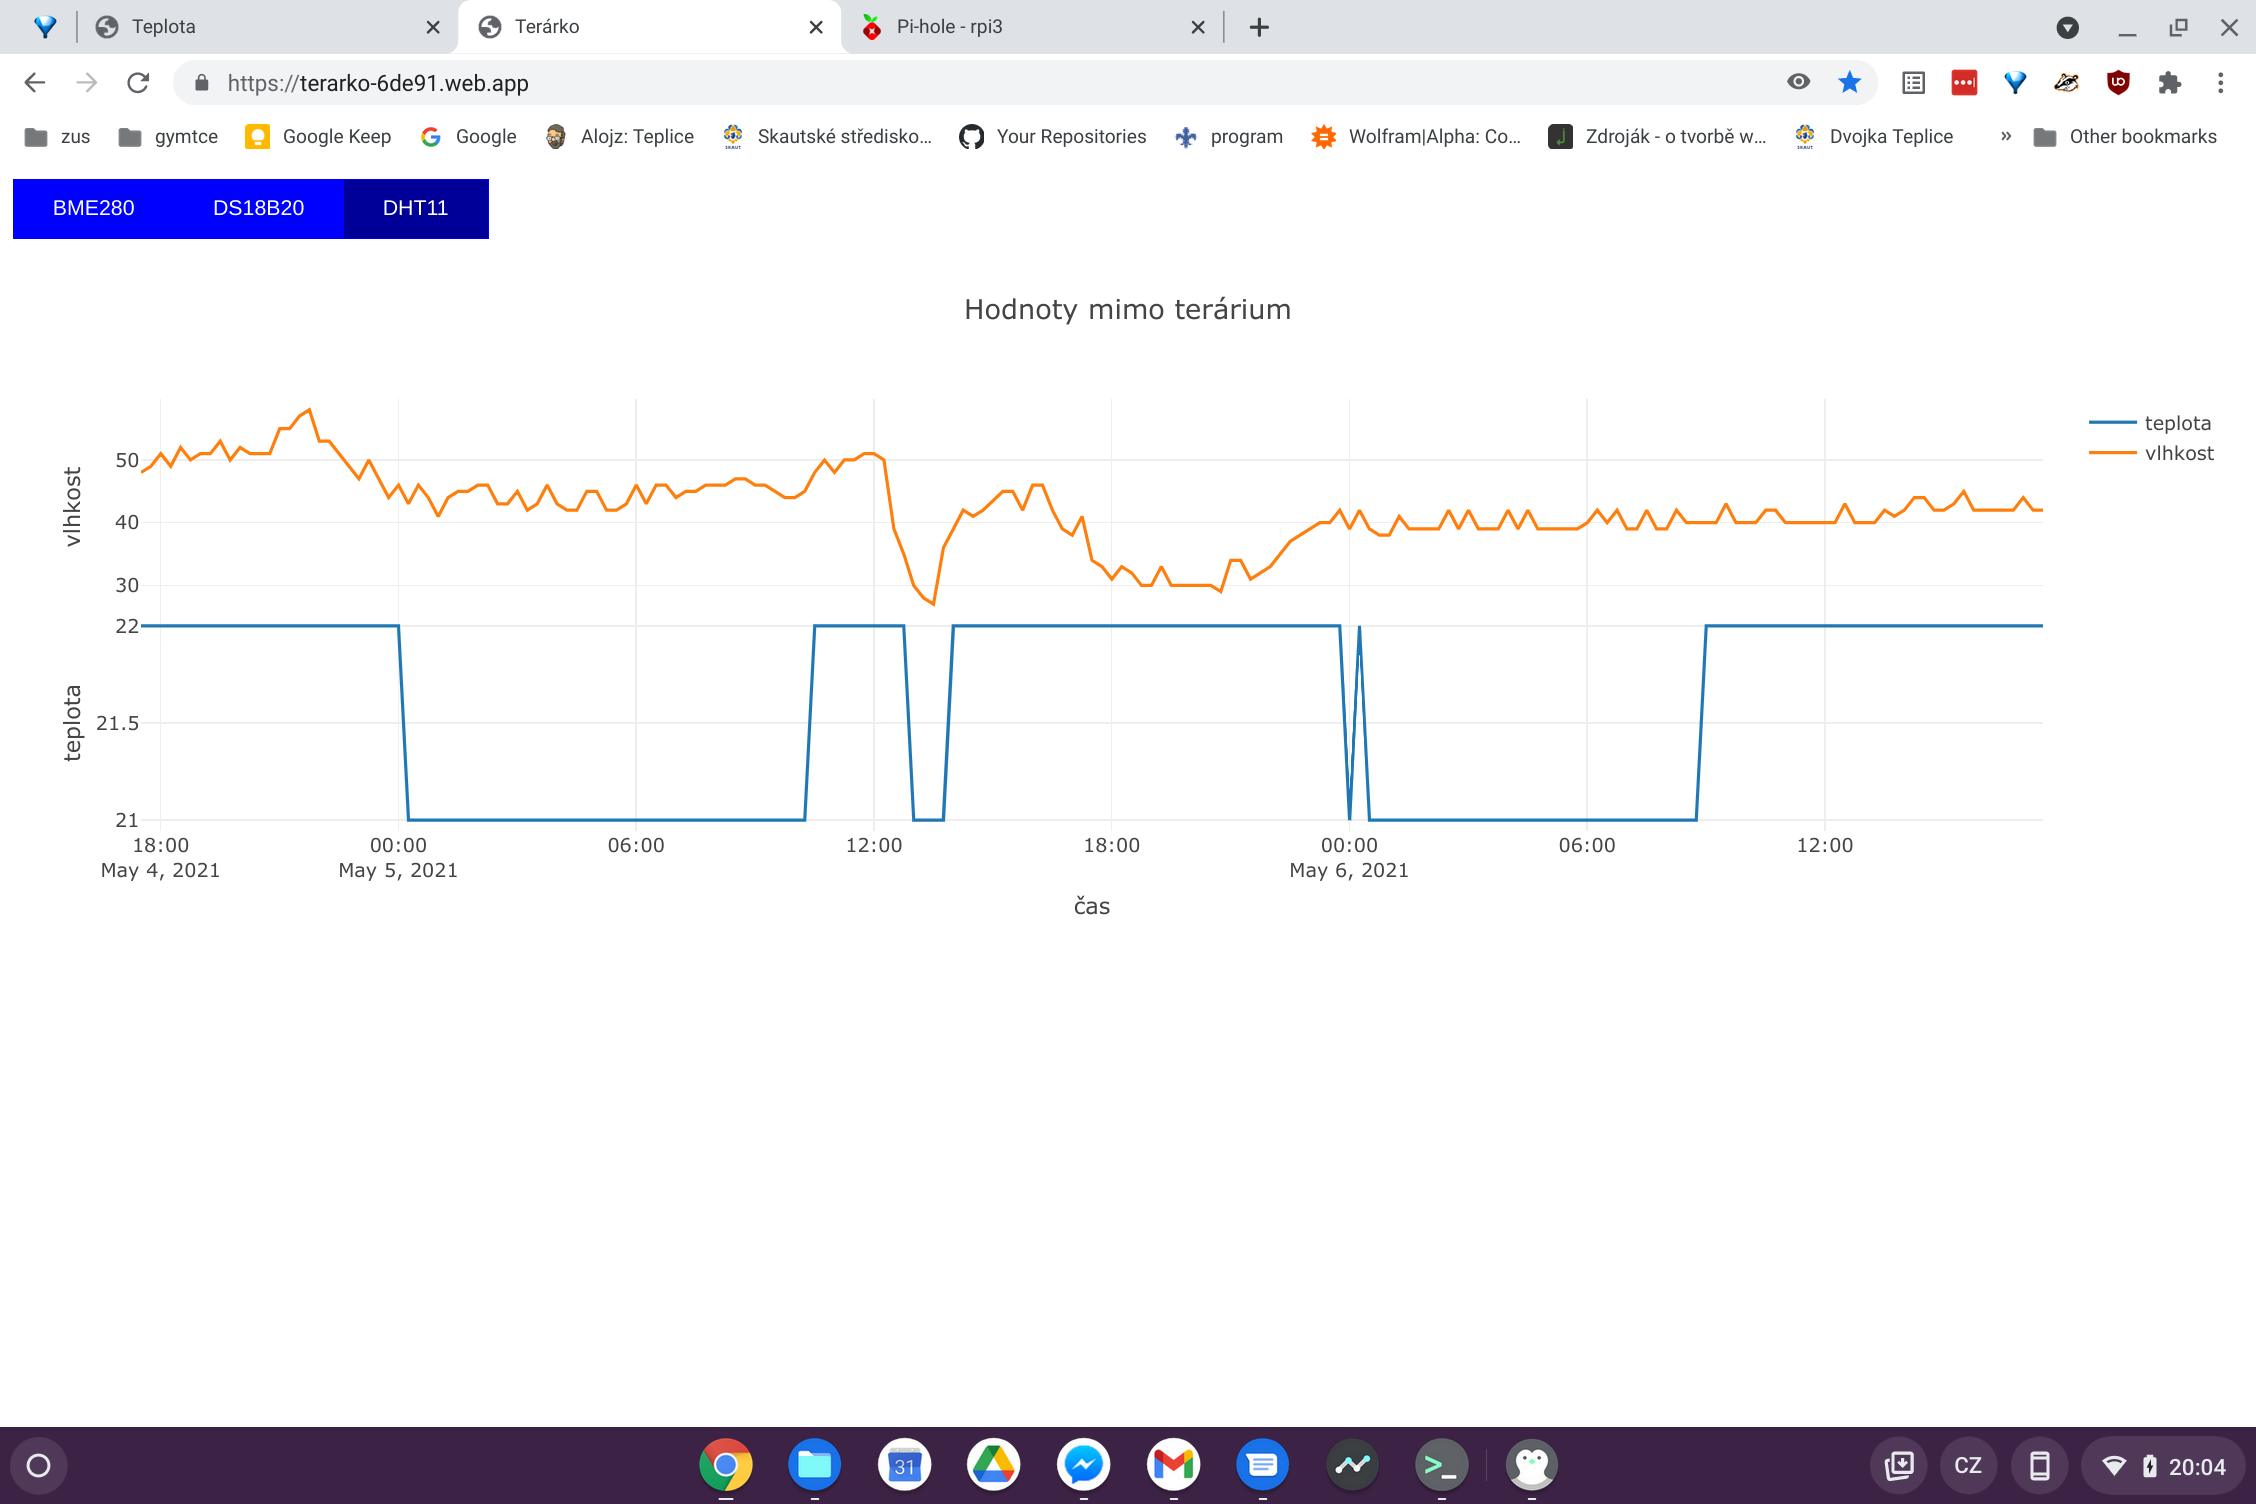
\includegraphics[width=0.8\textwidth]{DHT11-graf.png}
    \caption{Teplota a vlhkost mimo terárium}
\end{figure}
